\subsubsection{Aufbau von Schaltkreisen zur Lösung von Differentialgleichungen}

Im Folgenden werden zwei wesentliche Ansätze zum Ableiten eines analogen Computers von einer Reihe an Differentialgleichungen vorgestellt: die Kelvin Feedback Technik sowie die Substitutionsmethode.

Um einen analogen Rechner mithilfe der Kelvin Feedback Technik zu konstruieren, muss die vorliegende Differentialgleichungen so umgestellt werden, dass die höchsten Ableitungen alleine auf der linken Seite stehen. Die Ableitungen niedrigerem Grades können durch Integration der höchsten Ableitung gebildet werden, weshalb mithilfe der höchsten Ableitung die rechte Seite der Gleichung gebildet werden kann. Da die rechte Seite der Gleichung die höchste Ableitung darstellt, kann eine Rückkopplung hergestellt werden. \cite[vgl. S. 153 ff.]{Ulmann2022}

Die Substitutionsmethode substituiert Teile einer Gleichung, um Gleichungen ersten Grades zu erhalten. Die Schaltungen der substituierten Gleichungen werden verbunden, um das Ergebnis zu erhalten. Die Anwendung dieser Methode führt aber zu Schwierigkeiten beim Umgang mit Initialwerten ungleich null und ist umständlich für reale Anwendungen. \cite[vgl. S. 155 ff.]{Ulmann2022}

Der Wertebereich eines analogen Computers liegt i.d.R. bei \pm 1, weshalb Skalierung notwendig ist, um die berechneten Werte zu realen Werten umzuwandeln. Hierzu kann eine Zuordnung von maschinellen Variablen zu realen Variablen zum Einsatz kommen, jede Zuordnung ist dabei mit einem Skalierungsfaktor versehen. Die Skalierung von Zeit kann auch sinnvoll sein, um die Berechnungen zu beschleunigen. \cite[vgl. S. 162 ff.]{Ulmann2022}

Als Beispiel wird hier, wie von \cite[S. 168 ff.]{Ulmann2022} beschrieben, ein Masse-Feder-Dämpfer System aufgeführt:

Ein Gewicht mit einer Masse \(m\) ist mit einer Feder mit Starrheit \(s\) und einem Dämpfer mit Dämpfungsfaktor \(d\) verbunden. Sei \(y\) die Position des Gewichts, so wirkt durch das Gewicht die Kraft \(my''\), durch den Dämpfer \(dy'\) und durch die Feder \(sy\). Die Summe aller Kräfte in einem geschlossenem physikalischen System sind gleich 0, deshalb gilt:

\[my''+dy'+sy=0\]

Unter Anwendung der Kelvin Feedback Technik ergibt sich folgende Gleichung:

\[y''=\frac{-(dy'+sy)}{m}\]

Der Schaltkreis zur Lösung von \(-(dy'+sy)\) kann wie in Abbildung \ref{fig:Feder-Masse-Dämpfer System} gezeigt gebildet werden. Die Rückkopplung zu \(y''\) ist in Abbildung \ref{fig:Feder-Masse-Dämpfer System mit Rückkopplung} dargestellt.

\begin{figure}[h]
  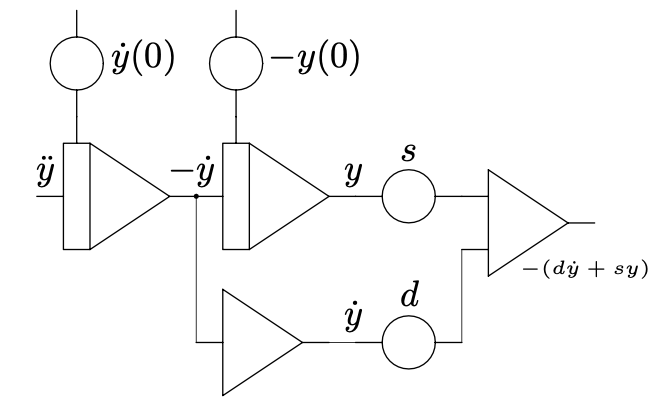
\includegraphics[width=0.5\textwidth]{abbildungen/feder_masse_daempfer.png}
  \caption{Masse-Feder-Dämpfer System ohne Rückkopplung. Quelle: \cite[S. 170]{Ulmann2022}}
  \label{fig:Feder-Masse-Dämpfer System}
\end{figure}

\begin{figure}[h]
  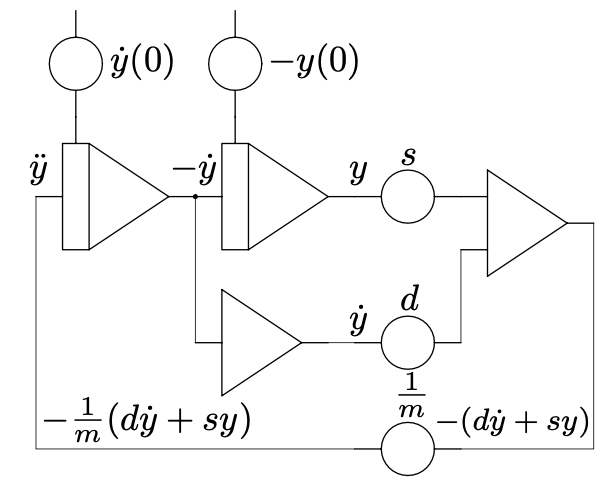
\includegraphics[width=0.5\textwidth]{abbildungen/feder_masse_daempfer_mit_rueckkopplung.png}
  \caption{Vollständiges Masse-Feder-Dämpfer System. Quelle: \cite[S. 170]{Ulmann2022}}
  \label{fig:Feder-Masse-Dämpfer System mit Rückkopplung}
\end{figure}

Zur Berechnung der realen Werte müssen die berechneten Werte entsprechend skaliert werden. Die Informationen über Maximalwerte von \(y\), \(y'\) und \(y''\) ist dafür notwendig.
